% answers.tex —— 2007 年·普通高等学校招生考试·福建卷·理科 · 参考答案与详细解析片段
% 由 tools/generate_projects.py 依来源总账自 2007/2007_数学真题_福建理_试题.md + 2007/2007_数学真题_福建理_解析正文.md + 2007/2007_数学真题_福建理_答案要点.md 生成，勿手改（改源 MD 后重跑）


\begin{gktip}
固定候选 PDF 仅含题面，无答案、解析和评分标准，原卷亦未标注分值；以下为非官方编者独立推导，官方答案字段为空。来源发布者、出版者、版次与官方身份均未核。
\end{gktip}

\begin{answer}
\gksolhead{1}{}

\textbf{题目}：

复数 $\dfrac1{(1+\mathrm i)^2}$ 等于（　）

（A）$\frac12$

（B）$-\frac12$

（C）$\frac12\mathrm i$

（D）$-\frac12\mathrm i$

\Needspace{4\baselineskip}
\textbf{解析}

\Needspace{5\baselineskip}
$(1+\mathrm i)^2=2\mathrm i$，故

\nopagebreak[4]
\[\frac1{(1+\mathrm i)^2}=\frac1{2\mathrm i}=\frac{-\mathrm i}2=-\frac12\mathrm i.\]

\gkanswer{答案：D。}

\end{answer}
\begin{answer}
\gksolhead{2}{}

\textbf{题目}：

数列 $\{a_n\}$ 的前 $n$ 项和为 $S_n$，若 $a_n=\dfrac1{n(n+1)}$，则 $S_5$ 等于（　）

（A）$1$

（B）$\frac56$

（C）$\frac16$

（D）$\frac1{30}$

\Needspace{4\baselineskip}
\textbf{解析}

\Needspace{5\baselineskip}
由 $a_n=\dfrac1{n(n+1)}=\dfrac1n-\dfrac1{n+1}$，得

\nopagebreak[4]
\[S_5=\left(1-\frac12\right)+\left(\frac12-\frac13\right)+\cdots+\left(\frac15-\frac16\right)=1-\frac16=\frac56.\]

\gkanswer{答案：B。}

\end{answer}
\begin{answer}
\gksolhead{3}{}

\textbf{题目}：

已知集合 $A=\{x\mid x<a\}$，$B=\{x\mid 1<x<2\}$，且 $A\cup(\complement_{\mathbf R}B)=\mathbf R$，则实数 $a$ 的取值范围是（　）

（A）$a\leqslant1$

（B）$a<1$

（C）$a\geqslant2$

（D）$a>2$

\Needspace{4\baselineskip}
\textbf{解析}

\Needspace{5\baselineskip}
$\complement_{\mathbf R}B=(-\infty,1]\cup[2,+\infty)$。$A=(-\infty,a)$，故

\nopagebreak[4]
\[A\cup(\complement_{\mathbf R}B)=\mathbf R\ \Longleftrightarrow\ (-\infty,a)\supset(1,2)\ \Longleftrightarrow\ a\geqslant2.\]

\gkanswer{答案：C。}

\end{answer}
\begin{answer}
\gksolhead{4}{}

\textbf{题目}：

对于向量 $\boldsymbol a$，$\boldsymbol b$，$\boldsymbol c$ 和实数 $\lambda$，下列命题中真命题的是（　）

（A）若 $\boldsymbol a\cdot\boldsymbol b=0$，则 $\boldsymbol a=\boldsymbol 0$ 或 $\boldsymbol b=\boldsymbol 0$

（B）若 $\lambda\boldsymbol a=\boldsymbol 0$，则 $\lambda=0$ 或 $\boldsymbol a=\boldsymbol 0$

（C）若 $\boldsymbol a^2=\boldsymbol b^2$，则 $\boldsymbol a=\boldsymbol b$ 或 $\boldsymbol a=-\boldsymbol b$

（D）若 $\boldsymbol a\cdot\boldsymbol b=\boldsymbol a\cdot\boldsymbol c$，则 $\boldsymbol b=\boldsymbol c$

\Needspace{4\baselineskip}
\textbf{解析}

（A）$\boldsymbol a\perp\boldsymbol b$ 时数量积为零而两向量均非零，假。

（B）$\lambda\boldsymbol a=\boldsymbol 0$ 时必有 $\lambda=0$ 或 $\boldsymbol a=\boldsymbol 0$，真。

（C）$\boldsymbol a^2=\boldsymbol b^2$ 只说明 $|\boldsymbol a|=|\boldsymbol b|$，假。

（D）只说明 $\boldsymbol a\perp(\boldsymbol b-\boldsymbol c)$，假。

\gkanswer{答案：B。}

\end{answer}
\begin{answer}
\gksolhead{5}{}

\textbf{题目}：

已知函数 $f(x)=\sin\left(\omega x+\dfrac{\pi}3\right)$（$\omega>0$）的最小正周期为 $\pi$，则该函数的图象（　）

（A）关于点 $\left(\dfrac{\pi}3,0\right)$ 对称

（B）关于直线 $x=\dfrac{\pi}4$ 对称

（C）关于点 $\left(\dfrac{\pi}4,0\right)$ 对称

（D）关于直线 $x=\dfrac{\pi}3$ 对称

\Needspace{4\baselineskip}
\textbf{解析}

由最小正周期 $\dfrac{2\pi}\omega=\pi$ 得 $\omega=2$，故 $f(x)=\sin\left(2x+\dfrac{\pi}3\right)$。

\Needspace{5\baselineskip}
$f\left(\dfrac{\pi}3\right)=\sin\pi=0$，且对任意 $t$，

\nopagebreak[4]
\[f\left(\frac{\pi}3+t\right)+f\left(\frac{\pi}3-t\right)=\sin(\pi+2t)+\sin(\pi-2t)=0,\]

故图象关于点 $\left(\dfrac{\pi}3,0\right)$ 对称。其余选项处函数值既不为 $0$ 也不为 $\pm1$，均不成立。

\gkanswer{答案：A。}

\end{answer}
\begin{answer}
\gksolhead{6}{}

\textbf{题目}：

以双曲线 $\dfrac{x^2}9-\dfrac{y^2}{16}=1$ 的右焦点为圆心，且与其渐近线相切的圆的方程是（　）

（A）$x^2+y^2-10x+9=0$

（B）$x^2+y^2-10x+16=0$

（C）$x^2+y^2+10x+16=0$

（D）$x^2+y^2+10x+9=0$

\Needspace{4\baselineskip}
\textbf{解析}

双曲线中 $a=3$，$b=4$，$c=5$，右焦点 $F(5,0)$，渐近线 $4x-3y=0$。

\Needspace{5\baselineskip}
圆心 $F$ 到渐近线的距离

\nopagebreak[4]
\[r=\frac{|4\times5-3\times0|}{\sqrt{4^2+3^2}}=4,\]

\Needspace{5\baselineskip}
故圆的方程为

\nopagebreak[4]
\[(x-5)^2+y^2=16\ \Longleftrightarrow\ x^2+y^2-10x+9=0.\]

\gkanswer{答案：A。}

\end{answer}
\begin{answer}
\gksolhead{7}{}

\textbf{题目}：

已知 $f(x)$ 为 $\mathbf R$ 上的减函数，则满足 $f\left(\left|\dfrac1x\right|\right)<f(1)$ 的实数 $x$ 的取值范围是（　）

（A）$(-1,1)$

（B）$(0,1)$

（C）$(-1,0)\cup(0,1)$

（D）$(-\infty,-1)\cup(1,+\infty)$

\Needspace{4\baselineskip}
\textbf{解析}

\Needspace{5\baselineskip}
$f$ 在 $\mathbf R$ 上递减，故

\nopagebreak[4]
\[f\left(\left|\frac1x\right|\right)<f(1)\ \Longleftrightarrow\ \left|\frac1x\right|>1\ \Longleftrightarrow\ \frac1{|x|}>1\ \Longleftrightarrow\ 0<|x|<1,\]

即 $x\in(-1,0)\cup(0,1)$。

\gkanswer{答案：C。}

\end{answer}
\begin{answer}
\gksolhead{8}{}

\textbf{题目}：

已知 $m$，$n$ 为两条不同的直线，$\alpha$，$\beta$ 为两个不同的平面，则下列命题中正确的是（　）

（A）$m\subset\alpha$，$n\subset\alpha$，$m\parallel\beta$，$n\parallel\beta\Rightarrow\alpha\parallel\beta$

（B）$\alpha\parallel\beta$，$m\subset\alpha$，$n\subset\beta\Rightarrow m\parallel n$

（C）$m\perp\alpha$，$m\perp n\Rightarrow n\parallel\alpha$

（D）$n\parallel m$，$n\perp\alpha\Rightarrow m\perp\alpha$

\Needspace{4\baselineskip}
\textbf{解析}

（A）当 $m\parallel n$ 时两平面仍可相交，假。

（B）两平行平面内的直线可以异面，假。

（C）$n$ 可能落在 $\alpha$ 内，假。

（D）$n\perp\alpha$ 且 $m\parallel n$，则 $m$ 的方向也是 $\alpha$ 的法方向，故 $m\perp\alpha$，真。

【源疑点：原页（D）印作「$n\parallel m$，$n\subset\alpha\Rightarrow m\perp\alpha$」，按字面四个选项无一成立；按命题意图与选项排布应为 $n\perp\alpha$，本库照 $n\perp\alpha$ 转录并作答，特此说明。文科卷第 9 题同一处亦为此形。】

\gkanswer{答案：D。}

\end{answer}
\begin{answer}
\gksolhead{9}{}

\textbf{题目}：

把 $1+(1+x)+(1+x)^2+\cdots+(1+x)^n$ 展开成关于 $x$ 的多项式，其各项系数和为 $a_n$，则 $\lim\limits_{n\to\infty}\dfrac{2a_n-1}{a_n+1}$ 等于（　）

（A）$\frac14$

（B）$\frac12$

（C）$1$

（D）$2$

\Needspace{4\baselineskip}
\textbf{解析}

\Needspace{5\baselineskip}
$1+(1+x)+\cdots+(1+x)^n$ 的各项系数和等于把 $x=1$ 代入所得的值：

\nopagebreak[4]
\[a_n=\sum_{k=0}^n2^k=2^{n+1}-1.\]

\Needspace{5\baselineskip}
于是

\nopagebreak[4]
\[\frac{2a_n-1}{a_n+1}=\frac{2^{n+2}-3}{2^{n+1}}=\frac{4-3\cdot2^{-n}}{2}\to2.\]

\gkanswer{答案：D。}

\end{answer}
\begin{answer}
\gksolhead{10}{}

\textbf{题目}：

顶点在同一球面上的正四棱柱 $ABCD-A'B'C'D'$ 中，$AB=1$，$AA'=\sqrt2$，则 $A$，$C$ 两点间的球面距离为（　）

（A）$\frac{\pi}4$

（B）$\frac{\pi}2$

（C）$\frac{\sqrt2}4\pi$

（D）$\frac{\sqrt2}2\pi$

\Needspace{4\baselineskip}
\textbf{解析}

\Needspace{5\baselineskip}
正四棱柱的底面是边长为 $1$ 的正方形，外接球球心在上下底面中心连线的中点。底面外接圆半径 $\dfrac{\sqrt2}2$，高的一半为 $\dfrac{\sqrt2}2$，故球半径

\nopagebreak[4]
\[R=\sqrt{\left(\frac{\sqrt2}2\right)^2+\left(\frac{\sqrt2}2\right)^2}=1.\]

\Needspace{5\baselineskip}
$A$，$C$ 是底面正方形的一对相对顶点，$AC=\sqrt2$。设球心角 $\angle AOC=\theta$，则

\nopagebreak[4]
\[\sin\frac\theta2=\frac{AC/2}{R}=\frac{\sqrt2/2}1=\frac{\sqrt2}2,\]

故 $\theta=\dfrac{\pi}2$，球面距离为 $R\theta=\dfrac{\pi}2$。

\gkanswer{答案：B。}

\end{answer}
\begin{answer}
\gksolhead{11}{}

\textbf{题目}：

已知对任意实数 $x$，有 $f(-x)=-f(x)$，$g(-x)=g(x)$，且 $x>0$ 时，$f'(x)>0$，$g'(x)>0$，则 $x<0$ 时，（　）

（A）$f'(x)>0$，$g'(x)>0$

（B）$f'(x)>0$，$g'(x)<0$

（C）$f'(x)<0$，$g'(x)>0$

（D）$f'(x)<0$，$g'(x)<0$

\Needspace{4\baselineskip}
\textbf{解析}

$f$ 为奇函数，导函数为偶函数：$f'(-x)=f'(x)$，故 $x<0$ 时 $f'(x)=f'(-x)>0$。

$g$ 为偶函数，导函数为奇函数：$g'(-x)=-g'(x)$，故 $x<0$ 时 $g'(x)=-g'(-x)<0$。

\gkanswer{答案：B。}

\end{answer}
\begin{answer}
\gksolhead{12}{}

\textbf{题目}：

\Needspace{5\baselineskip}
如图，三行三列的方阵中有 $9$ 个数 $a_{ij}$（$i=1,2,3$；$j=1,2,3$），从中任取三个数，则至少有两个数位于同行或同列的概率是（　）

\nopagebreak[4]
\[\begin{pmatrix}a_{11}&a_{12}&a_{13}\\ a_{21}&a_{22}&a_{23}\\ a_{31}&a_{32}&a_{33}\end{pmatrix}\]

（A）$\frac37$

（B）$\frac47$

（C）$\frac1{14}$

（D）$\frac{13}{14}$

\Needspace{4\baselineskip}
\textbf{解析}

\Needspace{5\baselineskip}
任取三个数共 $\mathrm C_9^3=84$ 种。“三个数两两不同行且不同列”等价于从三行三列中各取一个，共有 $3!=6$ 种（三种行与列的配对）。故至少两个数同行或同列的概率为

\nopagebreak[4]
\[P=1-\frac6{84}=1-\frac1{14}=\frac{13}{14}.\]

\gkanswer{答案：D。}

\end{answer}
\begin{answer}
\gksolhead{13}{}

\textbf{题目}：

已知实数 $x$，$y$ 满足 $\begin{cases}x+y\geqslant2,\\ x-y\leqslant2,\\ 0\leqslant y\leqslant3,\end{cases}$ 则 $z=2x-y$ 的取值范围是\gkblank{}。

\Needspace{4\baselineskip}
\textbf{解析}

\Needspace{5\baselineskip}
可行域顶点为 $(2,0)$、$(5,3)$、$(-1,3)$。计算 $z=2x-y$：

\nopagebreak[4]
\[4,\qquad 7,\qquad -5,\]

故取值范围是 $[-5,7]$。

\gkanswer{答案：$[-5,7]$。}

\end{answer}
\begin{answer}
\gksolhead{14}{}

\textbf{题目}：

已知正方形 $ABCD$，则以 $A$，$B$ 为焦点，且过 $C$，$D$ 两点的椭圆的离心率为\gkblank{}。

\Needspace{4\baselineskip}
\textbf{解析}

\Needspace{5\baselineskip}
设正方形边长为 $s$，以 $A$，$B$ 为焦点，则焦距

\nopagebreak[4]
\[2c=AB=s,\qquad c=\frac s2.\]

\Needspace{5\baselineskip}
$C$ 到两焦点的距离 $|CA|=s\sqrt2$，$|CB|=s$，故

\nopagebreak[4]
\[2a=|CA|+|CB|=s(1+\sqrt2),\qquad a=\frac{s(1+\sqrt2)}2.\]

\Needspace{5\baselineskip}
离心率

\nopagebreak[4]
\[e=\frac ca=\frac1{1+\sqrt2}=\sqrt2-1.\]

\gkanswer{答案：$\sqrt2-1$。}

\end{answer}
\begin{answer}
\gksolhead{15}{}

\textbf{题目}：

两封信随机投入 $A$，$B$，$C$ 三个空邮箱，则 $A$ 邮箱的信件数 $\xi$ 的数学期望 $E\xi=$\gkblank{}。

\Needspace{4\baselineskip}
\textbf{解析}

\Needspace{5\baselineskip}
每封信落入 $A$ 的概率为 $\dfrac13$，且两封信相互独立，故 $\xi\sim B\left(2,\dfrac13\right)$，

\nopagebreak[4]
\[E\xi=2\times\frac13=\frac23.\]

\gkanswer{答案：$\dfrac23$。}

\end{answer}
\begin{answer}
\gksolhead{16}{}

\textbf{题目}：

中学数学中存在许多关系，比如“相等关系”、“平行关系”等等。如果集合 $A$ 中元素之间的一个关系“$\sim$”满足以下三个条件：

① 自反性：对于任意 $a\in A$，都有 $a\sim a$；

② 对称性：对于 $a$，$b\in A$，若 $a\sim b$，则有 $b\sim a$；

③ 传递性：对于 $a$，$b$，$c\in A$，若 $a\sim b$，$b\sim c$，则有 $a\sim c$。

则称“$\sim$”是集合 $A$ 的一个等价关系。例如：“数的相等”是等价关系，而“直线的平行”不是等价关系（自反性不成立）。请你再列出三个等价关系：\gkblank{}。

\Needspace{4\baselineskip}
\textbf{解析}

三角形的全等关系、相似关系均满足自反性、对称性与传递性；整数的同余关系（同模 $n$ 的余数相同）同样满足三条性质。答案不唯一，任写三个即可。

\gkanswer{答案：例如：三角形的全等关系、三角形的相似关系、整数的同余关系。}

\end{answer}
\begin{answer}
\gksolhead{17}{}

\textbf{题目}：

在 $\triangle ABC$ 中，$\tan A=\dfrac14$，$\tan B=\dfrac35$。

（1）求角 $C$ 的大小；

（2）若 $AB$ 边的长为 $\sqrt{17}$，求 $BC$ 边的长。

\Needspace{4\baselineskip}
\textbf{解析}

\Needspace{5\baselineskip}
（1）由两角和的正切公式

\nopagebreak[4]
\[\tan(A+B)=\frac{\tan A+\tan B}{1-\tan A\tan B}=\frac{\frac14+\frac35}{1-\frac14\cdot\frac35}=\frac{\frac{17}{20}}{\frac{17}{20}}=1.\]

\Needspace{5\baselineskip}
$A$，$B$ 为三角形内角且正切为正，故 $A+B=45^\circ$，从而

\nopagebreak[4]
\[C=180^\circ-45^\circ=135^\circ.\]

\Needspace{5\baselineskip}
（2）由 $\tan A=\dfrac14$ 得 $\sin A=\dfrac1{\sqrt{17}}$。$AB=\sqrt{17}$ 为角 $C$ 的对边，由正弦定理

\nopagebreak[4]
\[\frac{BC}{\sin A}=\frac{AB}{\sin C},\]

\Needspace{5\baselineskip}
故

\nopagebreak[4]
\[BC=\sqrt{17}\cdot\frac{1/\sqrt{17}}{\sqrt2/2}=\sqrt2.\]

\gkanswer{答案：（1）$C=135^\circ$；（2）$BC=\sqrt2$。}

\end{answer}
\begin{answer}
\gksolhead{18}{}

\textbf{题目}：

如图，正三棱柱 $ABC-A_1B_1C_1$ 的所有棱长都为 $2$，$D$ 为 $CC_1$ 中点。

（1）求证：$AB_1\perp$ 平面 $A_1BD$；

（2）求二面角 $A-A_1D-B$ 的大小；

（3）求点 $C$ 到平面 $A_1BD$ 的距离。
\nopagebreak[4]
\begin{center}% 2007 年福建卷理科第 18 题：正三棱柱 ABC-A1B1C1（底面正三角形、侧棱垂直底面，
%   所有棱长均为 2），D 为 CC1 的中点；图中画出 AB1、A1B、A1D、BD 等辅助线。
% 来源 PDF：gaokaomath-src/普通高考/2007/2007福建理.pdf
% SHA-256：e9ade36d1b1e3154a7e37226957037a45635faeedcfb823df216fceabcc5a1dc
% 原页：2007福建理.pdf 第 1 页（A3 三栏）第 3 栏，书页码 367。
% 重绘依据：按原页横放的三棱柱（左三角面 ABC、右三角面 A1B1C1）与虚线重绘；
%   C 为被遮挡的后顶点，A-C、B-C、C-C1 画虚线，D 取 CC1 中点。
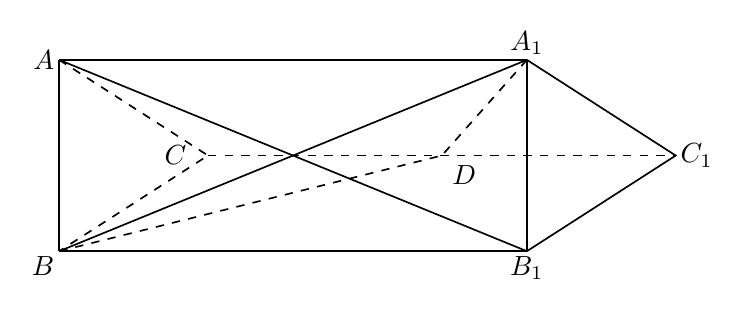
\begin{tikzpicture}[scale=0.9, semithick,
  every node/.style={inner sep=1.5pt}]

  \coordinate (A)  at (0.0,2.7);
  \coordinate (B)  at (0.0,0.0);
  \coordinate (C)  at (2.1,1.35);
  \coordinate (A1) at (6.6,2.7);
  \coordinate (B1) at (6.6,0.0);
  \coordinate (C1) at (8.7,1.35);
  \coordinate (D)  at (5.4,1.35);

  % 左三角面
  \draw (A) -- (B);
  \draw[dashed] (A) -- (C) -- (B);
  % 侧棱
  \draw (A) -- (A1);
  \draw (B) -- (B1);
  \draw[dashed] (C) -- (C1);
  % 右三角面
  \draw (A1) -- (B1);
  \draw (A1) -- (C1) -- (B1);
  % 题设辅助线
  \draw (A) -- (B1);
  \draw (A1) -- (B);
  \draw[dashed] (A1) -- (D);
  \draw[dashed] (B) -- (D);

  \node[left] at (A) {$A$};
  \node[below left] at (B) {$B$};
  \node[left=6pt] at (C) {$C$};
  \node[above] at (A1) {$A_1$};
  \node[below] at (B1) {$B_1$};
  \node[right] at (C1) {$C_1$};
  \node[below right=2pt] at (D) {$D$};
\end{tikzpicture}
\end{center}
\nopagebreak[4]
\Needspace{4\baselineskip}
\textbf{解析}

建立空间直角坐标系：取 $A(0,0,0)$，$B(2,0,0)$，$C(1,\sqrt3,0)$，$A_1(0,0,2)$，$B_1(2,0,2)$，$C_1(1,\sqrt3,2)$，$D(1,\sqrt3,1)$。

\Needspace{5\baselineskip}
（1）$\overrightarrow{AB_1}=(2,0,2)$。平面 $A_1BD$ 内

\nopagebreak[4]
\[\overrightarrow{A_1B}=(2,0,-2),\qquad \overrightarrow{A_1D}=(1,\sqrt3,-1),\]

\Needspace{5\baselineskip}
法向量

\nopagebreak[4]
\[\boldsymbol n=\overrightarrow{A_1B}\times\overrightarrow{A_1D}=\left(2\sqrt3,0,2\sqrt3\right)\parallel(1,0,1).\]

因 $\overrightarrow{AB_1}=2(1,0,1)\parallel\boldsymbol n$，故 $AB_1\perp$ 平面 $A_1BD$。

\Needspace{5\baselineskip}
（2）平面 $AA_1D$ 的法向量

\nopagebreak[4]
\[\boldsymbol n_1=\overrightarrow{AA_1}\times\overrightarrow{AD}=(0,0,2)\times(1,\sqrt3,1)=\left(-2\sqrt3,2,0\right)\parallel\left(-\sqrt3,1,0\right).\]

\Needspace{5\baselineskip}
平面 $A_1BD$ 的法向量 $\boldsymbol n_2=(1,0,1)$，故

\nopagebreak[4]
\[\cos\theta=\frac{\left|\boldsymbol n_1\cdot\boldsymbol n_2\right|}{\left|\boldsymbol n_1\right|\left|\boldsymbol n_2\right|}=\frac{\sqrt3}{2\sqrt2}=\frac{\sqrt6}4,\]

二面角 $A-A_1D-B$ 为 $\arccos\dfrac{\sqrt6}4$（约 $52.2^\circ$）。

【源疑点：原页第（2）问印作「二面角 $A-AD_1-B$」，题设只定义 $D$（$CC_1$ 中点）、图中无 $D_1$，按图形与第（1）问应为 $A-A_1D-B$，本库照此转录并作答。】

\Needspace{5\baselineskip}
（3）平面 $A_1BD$ 过 $A_1(0,0,2)$、法向量 $(1,0,1)$，方程为

\nopagebreak[4]
\[x+z-2=0.\]

\Needspace{5\baselineskip}
点 $C(1,\sqrt3,0)$ 到该平面的距离

\nopagebreak[4]
\[d=\frac{|1+0-2|}{\sqrt{1^2+1^2}}=\frac1{\sqrt2}=\frac{\sqrt2}2.\]

\gkanswer{答案：（1）证明见解析；（2）$\arccos\dfrac{\sqrt6}4$；（3）$\dfrac{\sqrt2}2$。}

\end{answer}
\begin{answer}
\gksolhead{19}{}

\textbf{题目}：

某分公司经销某种品牌产品，每件产品的成本为 $3$ 元，并且每件产品需向总公司交 $a$ 元（$3\leqslant a\leqslant5$）的管理费，预计当每件产品的售价为 $x$ 元（$9\leqslant x\leqslant11$）时，一年的销售量为 $(12-x)^2$ 万件。

（1）求分公司一年的利润 $L$（万元）与每件产品的售价 $x$ 的函数关系式；

（2）当每件产品的售价为多少元时，分公司一年的利润 $L$ 最大？并求出 $L$ 的最大值 $Q(a)$。

\Needspace{4\baselineskip}
\textbf{解析}

\Needspace{5\baselineskip}
（1）每件产品的利润为 $x-3-a$，故

\nopagebreak[4]
\[L=(x-3-a)(12-x)^2,\qquad 9\leqslant x\leqslant11.\]

\Needspace{5\baselineskip}
（2）令 $t=12-x\in[1,3]$，则 $x=12-t$，

\nopagebreak[4]
\[L=(9-a-t)t^2=(9-a)t^2-t^3.\]

\Needspace{5\baselineskip}
求导：

\nopagebreak[4]
\[L'(t)=2(9-a)t-3t^2=t\left(2(9-a)-3t\right).\]

驻点 $t_0=\dfrac{2(9-a)}3$。由 $3\leqslant a\leqslant5$ 得 $9-a\in[4,6]$，故 $t_0\in\left[\dfrac83,4\right]$。

\Needspace{5\baselineskip}
当 $3\leqslant a<\dfrac92$ 时 $t_0>3$，$L$ 在 $[1,3]$ 上递增，最大值在 $t=3$（即 $x=9$）处：

\nopagebreak[4]
\[Q(a)=L(3)=9(6-a)=54-9a.\]

\Needspace{5\baselineskip}
当 $\dfrac92\leqslant a\leqslant5$ 时 $t_0\in\left[\dfrac83,3\right]$，最大值在 $t=t_0$ 处：

\nopagebreak[4]
\[Q(a)=L(t_0)=t_0^2\left((9-a)-t_0\right)=\frac{4(9-a)^2}9\cdot\frac{9-a}3=\frac{4(9-a)^3}{27},\]

\Needspace{5\baselineskip}
此时

\nopagebreak[4]
\[x=12-t_0=12-\frac{2(9-a)}3=6+\frac{2a}3.\]

两段在 $a=\dfrac92$ 处都给出 $x=9$、$Q=\dfrac{27}2$，结论衔接。

\gkanswer{答案：（1）$L=(x-3-a)(12-x)^2$（$9\leqslant x\leqslant11$）；（2）$3\leqslant a\leqslant\dfrac92$ 时 $x=9$、$Q=54-9a$；$\dfrac92\leqslant a\leqslant5$ 时 $x=6+\dfrac{2a}3$、$Q=\dfrac{4(9-a)^3}{27}$。}

\end{answer}
\begin{answer}
\gksolhead{20}{}

\textbf{题目}：

如图，已知点 $F(1,0)$，直线 $l:x=-1$，$P$ 为平面上的动点，过 $P$ 作直线 $l$ 的垂线，垂足为点 $Q$，且 $\overrightarrow{QP}\cdot\overrightarrow{QF}=\overrightarrow{FP}\cdot\overrightarrow{FQ}$。

（1）求动点 $P$ 的轨迹 $C$ 的方程；

（2）过点 $F$ 的直线交轨迹 $C$ 于 $A$，$B$ 两点，交直线 $l$ 于点 $M$，已知 $\overrightarrow{MA}=\lambda_1\overrightarrow{AF}$，$\overrightarrow{MB}=\lambda_2\overrightarrow{BF}$，求 $\lambda_1+\lambda_2$ 的值。
\nopagebreak[4]
\begin{center}% 2007 年福建卷理科第 20 题：定点 F(1,0)、直线 l:x=-1，P 为动点，Q 为 P 在 l 上的
%   垂足，且 QP·QF = FP·FQ；第（2）问过 F 的直线交轨迹 C 于 A、B，交 l 于 M，求 λ1+λ2。
% 来源 PDF：gaokaomath-src/普通高考/2007/2007福建理.pdf
% SHA-256：e9ade36d1b1e3154a7e37226957037a45635faeedcfb823df216fceabcc5a1dc
% 原页：2007福建理.pdf 第 2 页（A3 三栏）第 1 栏，书页码 368。
% 重绘依据：按原页只画坐标轴、准线 l 与焦点 F，并在 x 轴上标出 -1 与 1。
\begin{tikzpicture}[x=0.85cm, y=0.85cm, semithick,
  every node/.style={inner sep=1.5pt}]

  % 坐标轴
  \draw[->,>=stealth] (-3.2,0) -- (4.2,0) node[right] {$x$};
  \draw[->,>=stealth] (0,-2.4) -- (0,3.0) node[above] {$y$};
  \node[below left] at (0,0) {$O$};

  % 直线 l：x=-1
  \draw (-1,-2.0) -- (-1,2.6) node[above] {$l$};

  % 焦点 F
  \fill (1,0) circle (1.3pt);
  \node[above right=1pt] at (1,0) {$F$};

  % x 轴上的刻度 -1、1
  \node[below] at (-1,0) {$-1$};
  \node[below] at (1,0) {$1$};
\end{tikzpicture}
\end{center}
\nopagebreak[4]
\Needspace{4\baselineskip}
\textbf{解析}

\Needspace{5\baselineskip}
（1）设 $P(x,y)$，则 $Q(-1,y)$。于是

\nopagebreak[4]
\[\overrightarrow{QP}=(x+1,0),\qquad \overrightarrow{QF}=(2,-y),\]

\nopagebreak[4]
\[\overrightarrow{FP}=(x-1,y),\qquad \overrightarrow{FQ}=(-2,y).\]

\Needspace{5\baselineskip}
由 $\overrightarrow{QP}\cdot\overrightarrow{QF}=\overrightarrow{FP}\cdot\overrightarrow{FQ}$ 得

\nopagebreak[4]
\[2(x+1)=-2(x-1)+y^2,\]

\Needspace{5\baselineskip}
化简得

\nopagebreak[4]
\[y^2=4x.\]

\Needspace{5\baselineskip}
（2）设过 $F(1,0)$ 的直线为 $y=k(x-1)$（$k\neq0$），与 $l:x=-1$ 交于

\nopagebreak[4]
\[M(-1,-2k).\]

\Needspace{5\baselineskip}
代入 $y^2=4x$：

\nopagebreak[4]
\[k^2x^2-(2k^2+4)x+k^2=0.\]

\Needspace{5\baselineskip}
设 $A(x_1,y_1)$，$B(x_2,y_2)$，则

\nopagebreak[4]
\[x_1+x_2=2+\frac4{k^2},\qquad x_1x_2=1.\]

\Needspace{5\baselineskip}
由 $\overrightarrow{MA}=\lambda_1\overrightarrow{AF}$ 比较横坐标：$x_1+1=\lambda_1(1-x_1)$，故

\nopagebreak[4]
\[\lambda_1=\frac{x_1+1}{1-x_1};\]

\Needspace{5\baselineskip}
同理 $\lambda_2=\dfrac{x_2+1}{1-x_2}$。于是

\nopagebreak[4]
\[\lambda_1+\lambda_2=\frac{(x_1+1)(1-x_2)+(x_2+1)(1-x_1)}{(1-x_1)(1-x_2)}=\frac{2-2x_1x_2}{1-(x_1+x_2)+x_1x_2}.\]

\Needspace{5\baselineskip}
代入 $x_1x_2=1$ 得分子为 $0$、分母为 $1-(x_1+x_2)+1\neq0$，故

\nopagebreak[4]
\[\lambda_1+\lambda_2=0.\]

\gkanswer{答案：（1）$y^2=4x$；（2）$0$。}

\end{answer}
\begin{answer}
\gksolhead{21}{}

\textbf{题目}：

等差数列 $\{a_n\}$ 的前 $n$ 项和为 $S_n$，$a_1=1+\sqrt2$，$S_3=9+3\sqrt2$。

（1）求数列 $\{a_n\}$ 的通项 $a_n$ 与前 $n$ 项和为 $S_n$；

（2）设 $b_n=\dfrac{S_n}n$（$n\in\mathbf N^*$），求证：数列 $\{b_n\}$ 中任意不同的三项都不可能成为等比数列。

\Needspace{4\baselineskip}
\textbf{解析}

\Needspace{5\baselineskip}
（1）设公差为 $d$，由 $S_3=3a_1+3d$：

\nopagebreak[4]
\[3(1+\sqrt2)+3d=9+3\sqrt2\ \Longrightarrow\ d=2.\]

\Needspace{5\baselineskip}
故

\nopagebreak[4]
\[a_n=1+\sqrt2+2(n-1)=2n-1+\sqrt2,\]

\nopagebreak[4]
\[S_n=\frac{n(a_1+a_n)}2=\frac{n\left[(1+\sqrt2)+(2n-1+\sqrt2)\right]}2=n(n+\sqrt2).\]

（2）$b_n=\dfrac{S_n}n=n+\sqrt2$。

\Needspace{5\baselineskip}
反设存在不同的三项 $b_i$，$b_j$，$b_k$（$i<j<k$）成等比数列，则

\nopagebreak[4]
\[(j+\sqrt2)^2=(i+\sqrt2)(k+\sqrt2),\]

\Needspace{5\baselineskip}
即

\nopagebreak[4]
\[j^2+2\sqrt2 j+2=ik+\sqrt2(i+k)+2,\]

\nopagebreak[4]
\[j^2-ik+\sqrt2\left(2j-i-k\right)=0.\]

\Needspace{5\baselineskip}
由 $i$，$j$，$k$ 均为整数、$\sqrt2$ 为无理数，得

\nopagebreak[4]
\[j^2=ik,\qquad 2j=i+k.\]

于是 $i$，$k$ 是方程 $t^2-2jt+j^2=0$ 的两根，即 $(t-j)^2=0$，故 $i=k=j$，与三项互不相同矛盾。

所以 $\{b_n\}$ 中任意不同的三项都不可能成为等比数列。

\gkanswer{答案：（1）$a_n=2n-1+\sqrt2$，$S_n=n(n+\sqrt2)$；（2）证明见解析。}

\end{answer}
\begin{answer}
\gksolhead{22}{}

\textbf{题目}：

已知函数 $f(x)=\mathrm e^x-kx$，$x\in\mathbf R$。

（1）若 $k=\mathrm e$，试确定函数 $f(x)$ 的单调区间；

（2）若 $k>0$，且对于任意 $x\in\mathbf R$，$f(|x|)>0$ 恒成立，试确定实数 $k$ 的取值范围；

（3）设函数 $F(x)=f(x)+f(-x)$，求证：$F(1)F(2)\cdots F(n)>(\mathrm e^{n+1}+2)^{\frac n2}$（$n\in\mathbf N^*$）。

\Needspace{4\baselineskip}
\textbf{解析}

\Needspace{5\baselineskip}
（1）$k=\mathrm e$ 时

\nopagebreak[4]
\[f'(x)=\mathrm e^x-\mathrm e.\]

$x<1$ 时 $f'(x)<0$，$x>1$ 时 $f'(x)>0$，故 $f$ 在 $(-\infty,1)$ 上递减，在 $(1,+\infty)$ 上递增。

（2）$f(|x|)>0$ 对一切 $x$ 成立，等价于 $t\geqslant0$ 时 $f(t)>0$。

$f'(t)=\mathrm e^t-k$。若 $0<k\leqslant1$，则 $t\geqslant0$ 时 $f'(t)\geqslant0$，$f(t)\geqslant f(0)=1>0$，符合要求。

\Needspace{5\baselineskip}
若 $k>1$，则 $t=\ln k$ 为最小值点，

\nopagebreak[4]
\[f(\ln k)=k-k\ln k=k(1-\ln k)>0\ \Longleftrightarrow\ \ln k<1\ \Longleftrightarrow\ k<\mathrm e.\]

综上，$0<k<\mathrm e$。

\Needspace{5\baselineskip}
（3）

\nopagebreak[4]
\[F(x)=f(x)+f(-x)=\mathrm e^x+\mathrm e^{-x}.\]

\Needspace{5\baselineskip}
对 $k=1,2,\cdots,n$，把第 $k$ 项与第 $n+1-k$ 项配对：

\nopagebreak[4]
\[\left(\mathrm e^k+\mathrm e^{-k}\right)\left(\mathrm e^{n+1-k}+\mathrm e^{-(n+1-k)}\right)
=\mathrm e^{n+1}+\mathrm e^{-(n+1)}+\mathrm e^{2k-n-1}+\mathrm e^{n+1-2k}.\]

\Needspace{5\baselineskip}
由均值不等式 $\mathrm e^{2k-n-1}+\mathrm e^{n+1-2k}\geqslant2$，且 $\mathrm e^{-(n+1)}>0$，故每一对之积

\nopagebreak[4]
\[> \mathrm e^{n+1}+2.\]

\Needspace{5\baselineskip}
当 $n$ 为偶数时共 $\dfrac n2$ 对，直接得

\nopagebreak[4]
\[F(1)F(2)\cdots F(n)>\left(\mathrm e^{n+1}+2\right)^{n/2}.\]

\Needspace{5\baselineskip}
当 $n$ 为奇数时，余下中间一项 $k=\dfrac{n+1}2$：

\nopagebreak[4]
\[F\left(\frac{n+1}2\right)=\mathrm e^{(n+1)/2}+\mathrm e^{-(n+1)/2}>\sqrt{\mathrm e^{n+1}+2},\]

\Needspace{5\baselineskip}
因为两边平方后 $\mathrm e^{n+1}+2+\mathrm e^{-(n+1)}>\mathrm e^{n+1}+2$。故

\nopagebreak[4]
\[F(1)F(2)\cdots F(n)>\left(\mathrm e^{n+1}+2\right)^{(n-1)/2}\cdot\left(\mathrm e^{n+1}+2\right)^{1/2}=\left(\mathrm e^{n+1}+2\right)^{n/2}.\]

综上，对一切 $n\in\mathbf N^*$，所证不等式成立。

\gkanswer{答案：（1）减区间 $(-\infty,1)$，增区间 $(1,+\infty)$；（2）$0<k<\mathrm e$；（3）证明见解析。}

\end{answer}